\section{Chaotic system under study}
\label{sec:chaos}

The  family of $2D$-quadratic maps studied here is given by the
 above equation \ref{eq:mapaSprott}.The $12D$ parameters space generated by coefficients $A=\{a_1,...,a_{12}\}$  is very hard to be explored. But Sprott
discovered that this set of equations produce a huge number of
chaotic attractors (about $6 .  10^{16}$) in floating-point
arithmetic. Three of these chaotic attractors are shown together in Fig. \ref{fig:atractores}. Their parameters sets $A_i$ are:
%
\begin{enumerate}[a)]
\item  $A_1=\{-0.7,~-0.4,~0.5,~-1.0,~ -0.9,~ -0.8, ~0.5, ~0.5,~0.3,~0.9,~-0.1,\\
~~~~~~~  ~-0.9\}$,
\item $A_2=\{-0.6,~-0.1,~1.1,~0.2,~-0.8,~0.6,~-0.7,~0.7,~0.7,~0.3,~0.6,~0.9\}$, 
\item $A_3=\{ -0.1,~ 0.8,~ -0.7,~ -1.1,~1.1,~-0.7,~-0.4,~ 0.6,~ -0.6,~-0.3,~1.2,~0.6\}$.
\end{enumerate}
%

Figures \ref{fig:atractores3592}.a to \ref{fig:atractores3592}.d show the same three attractors $A_1$ to $A_3$  and also the attractor with $A_4=\{-1,0.9,0.4,-0.2,-0.6,-0.5,0.4,0.7,0.3,-0.5,0.7,-0.8\}$, superimposed with their basins of attraction (in grey).  The white areas of each figure correspond to 
those initial conditions generating divergent trajectories of the system.

%%=========================ATRACTORES 3, 5 y 9 JUNTOS =======================================
\begin{figure}
    \centering
    \includegraphics[width=1\columnwidth]{atractoreslindos}\\
    \caption{Three attractors for three different sets of  coefficients of $2D$-quadratic map.}\label{fig:atractores}
\end{figure}
%===========================================================================================
%
%==========================ATRACTORES 3, 5, 8 Y 2 CON SUS DOMINIOS============================
\begin{figure}
\begin{tabular}{cc}
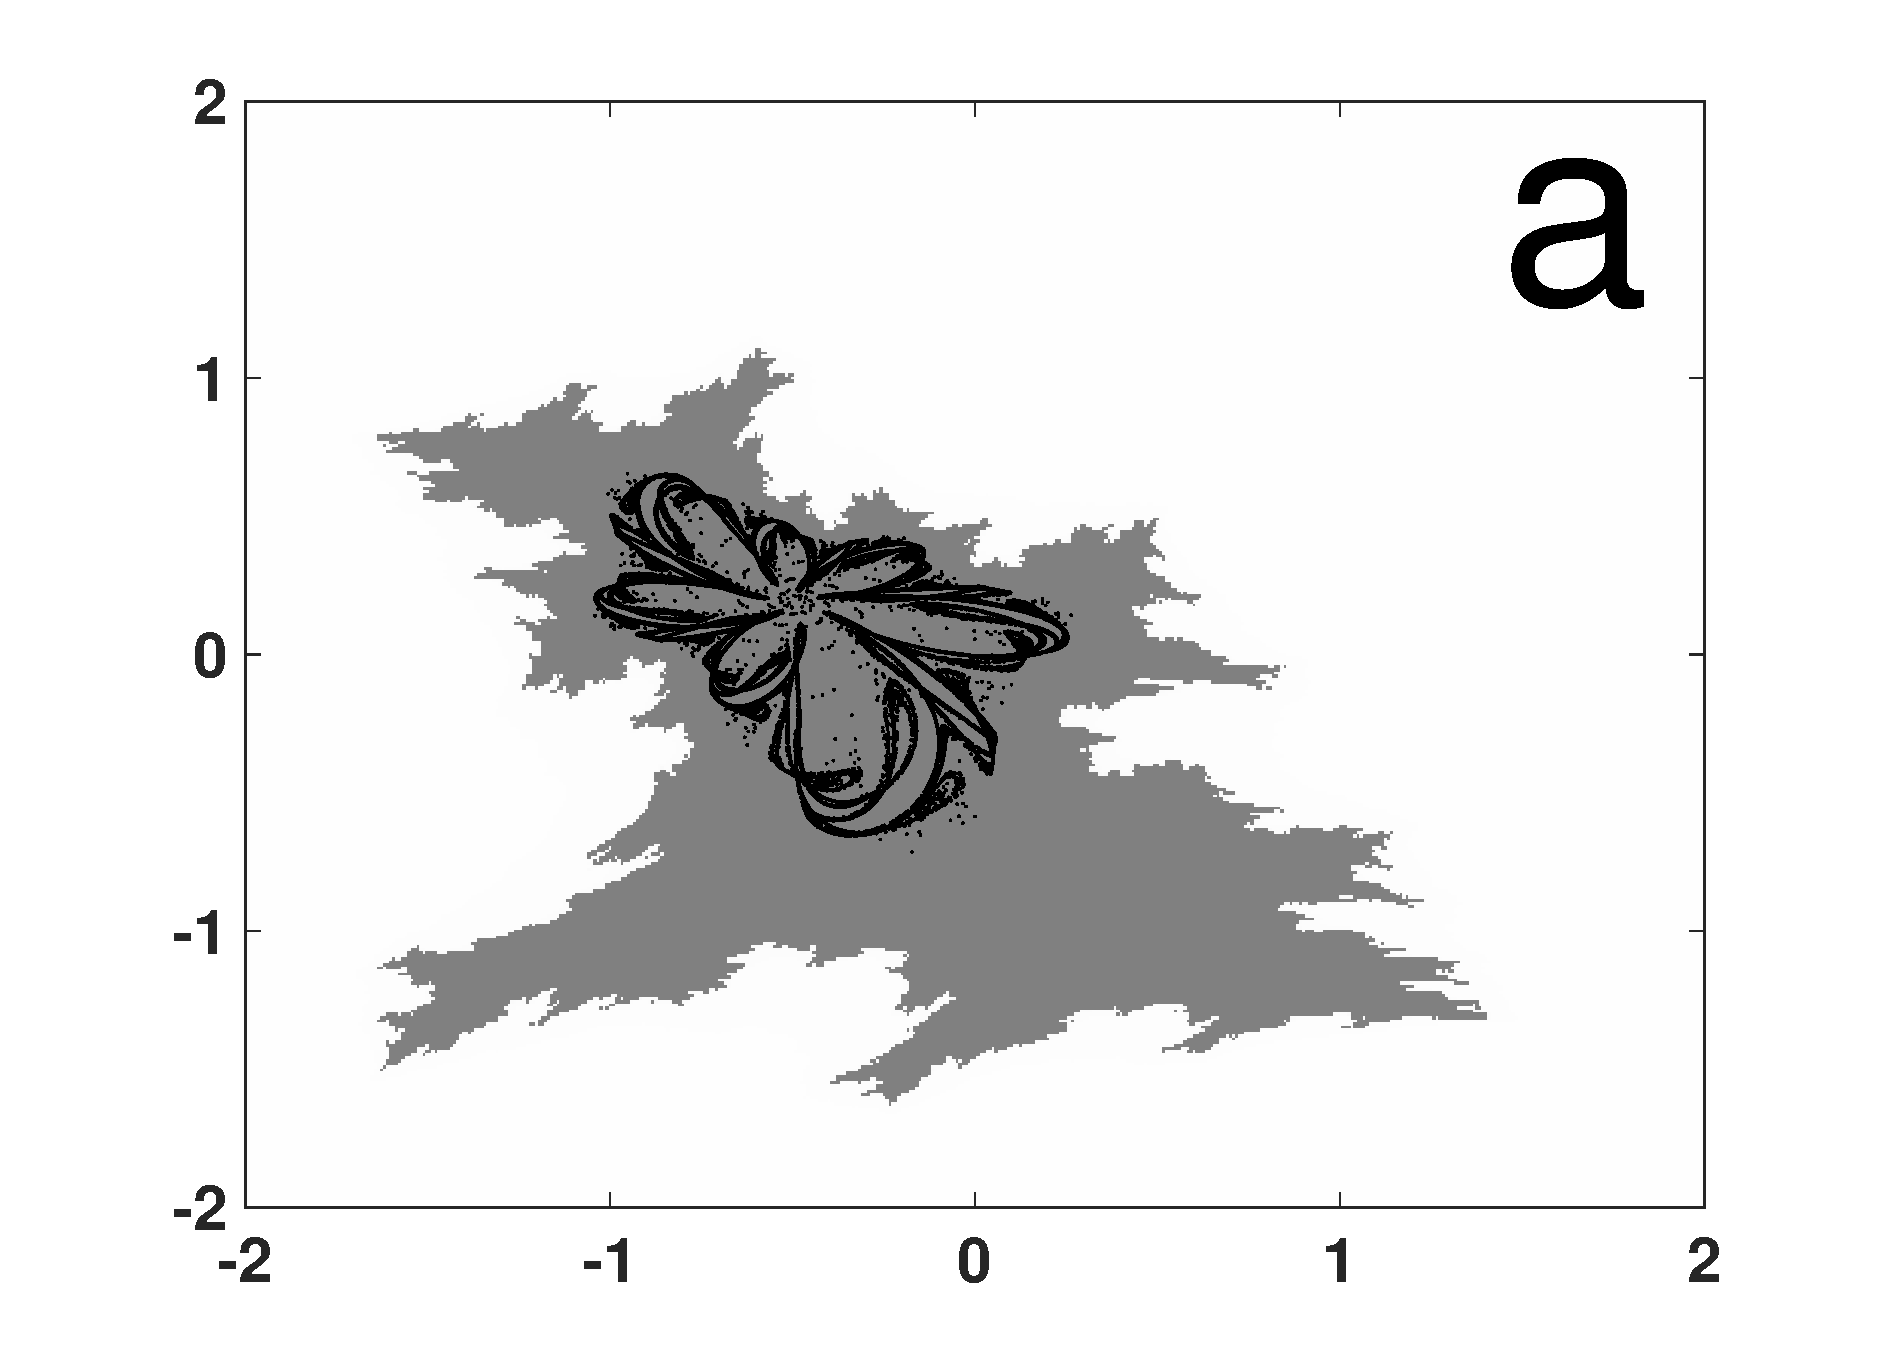
\includegraphics[width=0.5\textwidth]{Atractor3_condominio_ok}
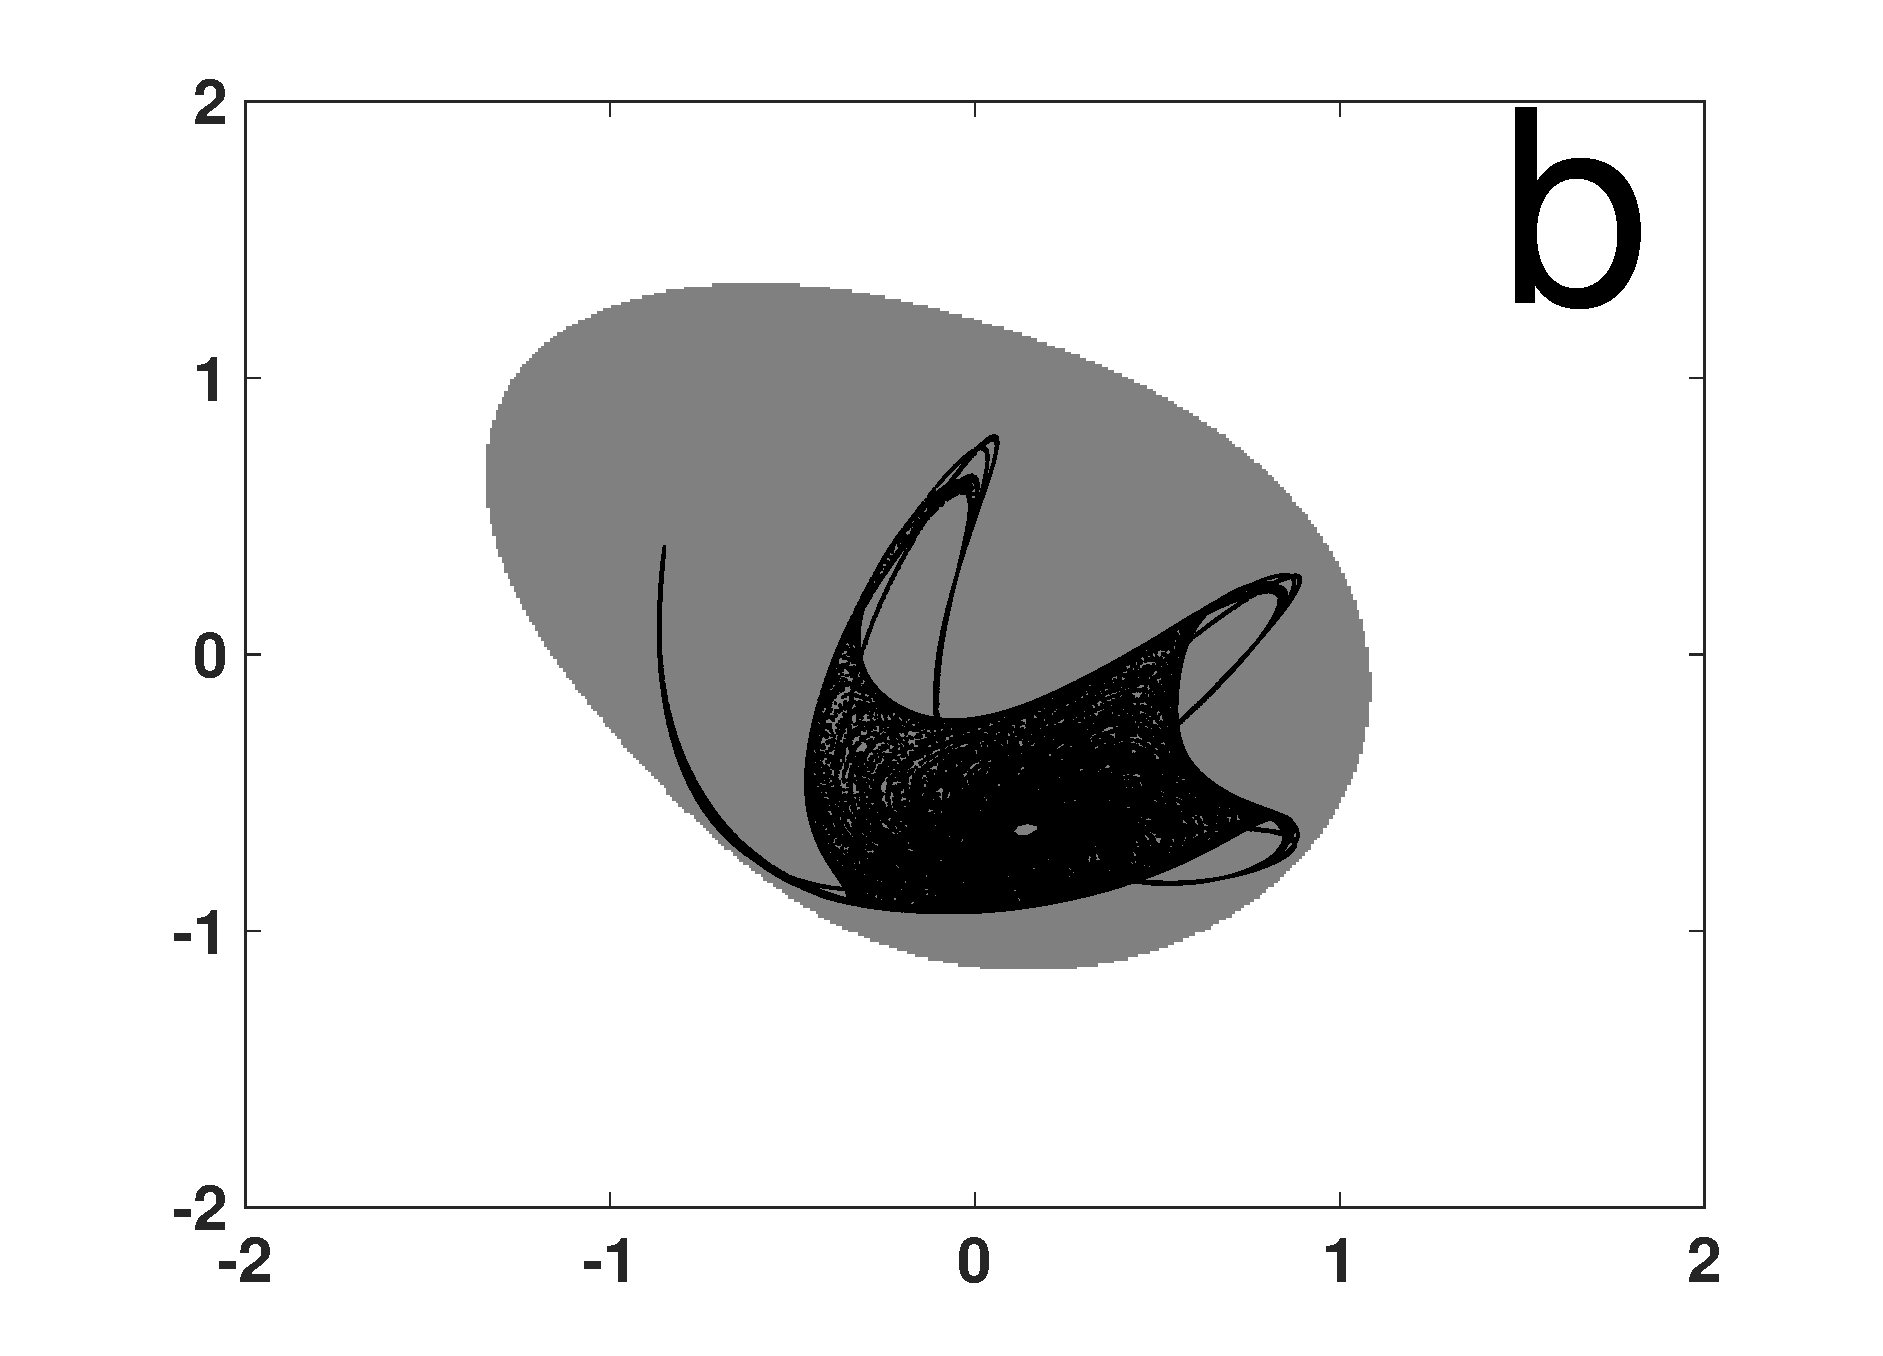
\includegraphics[width=0.5\textwidth]{Atractor5_condominio_ok}\\
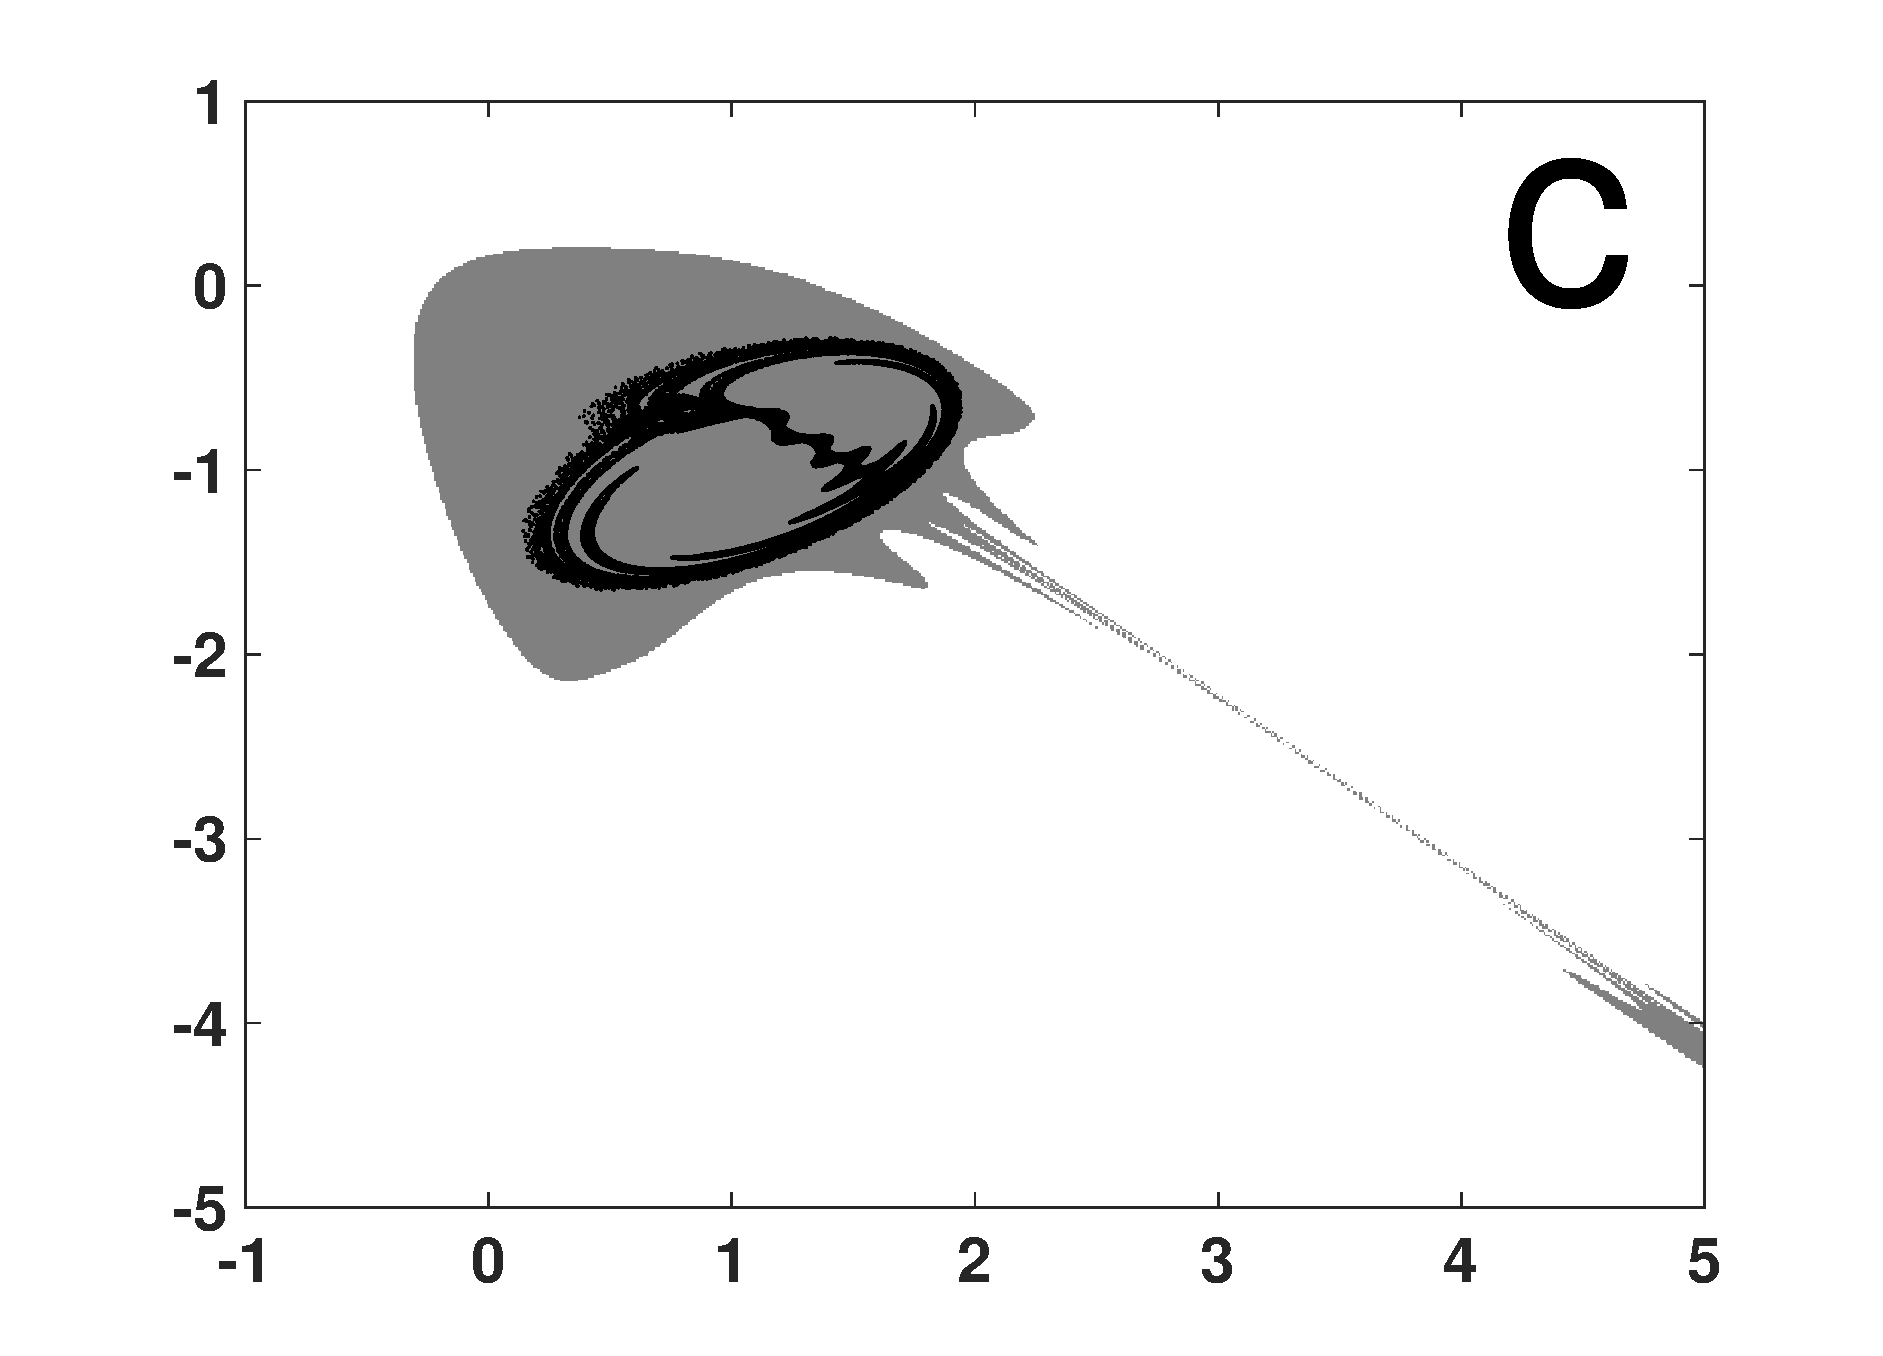
\includegraphics[width=0.5\textwidth]{Atractor9_condominio_ok}
\includegraphics[width=0.5\textwidth]{Atractor2_condominio_ok}
\end{tabular}
\caption{Four chaotic attractors and their domains of attraction in floating-point arithmetics. The set of parameters are (see text):
(a) $\{a_i\}=A_1$; (b)  $\{a_i\}=A_2$; (c)  $\{a_i\}=A_3$;  (d) $\{a_i\}=A_4$, \cite{Sprott1993}.}
\label{fig:atractores3592}
\end{figure}